%%%%%%%%%%%%%%%%%%%%%%%%%%%%%%%%%%%%%%%%%%%%%%%%%%%%%%%%%%%%%%%%%%%%%%%%%%%%%%%%
% event_selection.tex: 
%%%%%%%%%%%%%%%%%%%%%%%%%%%%%%%%%%%%%%%%%%%%%%%%%%%%%%%%%%%%%%%%%%%%%%%%%%%%%%%%
\chapter{Event Selection}
\label{sec:event_selection_chapter}
%%%%%%%%%%%%%%%%%%%%%%%%%%%%%%%%%%%%%%%%%%%%%%%%%%%%%%%%%%%%%%%%%%%%%%%%%%%%%%%%

LRS models presented earlier predict the existence of a \WR boson and heavy neutrinos \nul, and that their 
production and decay yields events with two high energy jets and two high energy charged leptons.  Using 
the 2.6 fb$^{-1}$ \cite{lumi} of data recorded by CMS from September through November 2015, evidence of 
\WR and \nul production was searched for in events with $\ell\ell jj$ ($\ell = e,\mu$) final states.  
Events were selected using lepton and jet selections developed from features of ST backgrounds 
and $\WR \rightarrow \ell\nul \rightarrow \ell\ell jj$ decays.


\section{\WR and \nul Signal Features}
\label{sec:signalFeatures}
Lepton and jet selections were driven by model independent features of \WR and \nul decays, and characteristics 
of ST backgrounds.  The expected \WR mass 
(\mWR) was large, above 2 $\TeV$, relative to the 13 $\TeV$ collision energy, 
so \WR bosons were expected to have low net momentum.  Therefore, the charged lepton and jet decay 
products, on average, were distributed uniformly in $\phi$, and concentrated in the region $|\eta| < 2.4$, 
as shown in Figures \ref{fig:wrLeptonEtas} and \ref{fig:wrJetEtas}.  Furthermore, the large expected 
\mWR meant final state leptons and jets would each have $\pt$ of several hundred $\GeV$ or more, as shown in 
Figures \ref{fig:wrLeptonPts} and \ref{fig:wrJetPts}.  In contrast, the majority of ST background events 
produced leptons and jets with $\pt$ below 100 $\GeV$.  The lepton and jet kinematic distributions, and 
the large expected \mWR motivated the following event selections:

\begin{itemize}
	\item Two leptons were reconstructed with $\pt > 53$ $\GeV$, and one had $\pt > 60$ $\GeV$.
	\item Two jets were reconstructed with $\pt > 40$ $\GeV$.
	\item Both leptons and jets were reconstructed with $|\eta| < 2.4$.
	\item The invariant mass $\Mlljj$ of the reconstructed leptons and jets exceeded $\Mlljj > 600$ $\GeV$.
\end{itemize}

The large expected mass difference between any charged lepton $\ell$ and heavy neutrino \nul motivated 
additional selections.  To conserve momentum in the $\WR \rightarrow \ell_{1} \nul$ 
decay, $\ell_{1}$ recoiled against the neutrino \nul.  Then the \nul decayed to 
$\ell_{2}$ and two jets, which recoiled against $\ell_{1}$.  Thus the lepton pair $\ell_{1}\ell_{2}$, 
on average, had a large dilepton mass $\Mll$ (Table \ref{tab:wrMll}), and $\ell_{1}$ was well separated 
from the \nul decay 
products (Figure \ref{fig:wrLeadLeptJetSeparation}).  In addition, the large expected neutrino mass \mnul, hundreds of 
$\GeV$ or more, needed to predict low ST neutrino masses resulted in large separations 
between $\ell_{2}$ and both jets, as shown in Figure \ref{fig:wrSubleadLeptJetSeparation}.  In contrast, \DY 
and diboson (WW, WZ, ZZ) background events primarily had $\Mll < 180 \GeV$, and in 
QCD multi-jet background events with a reconstructed lepton, the lepton was often close to a reconstructed 
jet.  The separation between leptons and jets, and the recoil of $\ell_{1}$ against $\ell_{2}$ motivated 
additional event selections:

\begin{itemize}
	\item Each reconstructed lepton was separated from the other lepton and both jets by $\Delta R > 0.4$.
	\item The dilepton mass $\Mll$ of the two reconstructed leptons exceeded $\Mll > 200$ $\GeV$.
\end{itemize}


\begin{figure}[btp]
	\centering
	\subfigure{
		
\includegraphics[width=0.65\textwidth]{figures/missingImage.png}
	}
	\subfigure{
		
\includegraphics[width=0.65\textwidth]{figures/missingImage.png}
	}
	\label{fig:wrLeptonEtas}
	\caption{The $\eta$ distribution of the leading (sub-leading) reconstructed muon is shown on the left (right) for 
		$\WR \rightarrow \mu\mu jj$ events with $\mWR = 2.0 \TeV$ and $\mnul = 1.0 \TeV$.  The electron 
	distributions are identical, except for the ECAL barrel-endcap gap where electrons are not reconstructed.}
\end{figure}

\begin{figure}[btp]
	\centering
	\subfigure{
		
\includegraphics[width=0.65\textwidth]{figures/missingImage.png}
	}
	\subfigure{
		
\includegraphics[width=0.65\textwidth]{figures/missingImage.png}
	}
	\label{fig:wrJetEtas}
	\caption{The $\eta$ distribution of the leading (sub-leading) reconstructed jet is shown on the left (right) for 
		$\WR \rightarrow \mu\mu jj$ events with $\mWR = 2.0 \TeV$ and $\mnul = 1.0 \TeV$.}
\end{figure}

\begin{figure}[btp]
	\centering
	\subfigure{
		
\includegraphics[width=0.65\textwidth]{figures/missingImage.png}
	}
	\subfigure{
		
\includegraphics[width=0.65\textwidth]{figures/missingImage.png}
	}
	\label{fig:wrLeptonPts}
	\caption{The $\pt$ distribution of the leading (sub-leading) reconstructed muon is shown on the left (right) for 
		$\WR \rightarrow \mu\mu jj$ events with $\mWR = 2.0 \TeV$ and $\mnul = 1.0 \TeV$.}
\end{figure}

\begin{figure}[btp]
	\centering
	\subfigure{
		
\includegraphics[width=0.65\textwidth]{figures/missingImage.png}
	}
	\subfigure{
		
\includegraphics[width=0.65\textwidth]{figures/missingImage.png}
	}
	\label{fig:wrJetPts}
	\caption{The $\pt$ distribution of the leading (sub-leading) reconstructed jet is shown on the left (right) for 
		$\WR \rightarrow \mu\mu jj$ events with $\mWR = 2.0 \TeV$ and $\mnul = 1.0 \TeV$.}
\end{figure}

\begin{table}[h]
	\caption{Fraction of expected $\WR \rightarrow \ell\ell jj$ events with dilepton mass $\Mll > 200$ \GeV. ($\mnul = \frac{1}{2}\mWR$)}
	\label{tab:wrMll}
	\centering
	\begin{tabular}{c|c}
		\mWR (\TeV) & Fraction of events with high \Mll (\%) \\  \hline
		1.0 &  88.  \\
		2.0 &  98.  \\
		3.0 &  99.  \\ \hline
	\end{tabular}
\end{table}

%\begin{figure}[btp]
%	\centering
%	
\includegraphics[width=0.65\textwidth]{figures/missingImage.png}
%	\label{fig:wrSigMll}
%	\caption{The dilepton mass $\Mll$ distribution for $\WR \rightarrow \mu\mu jj$ events with 
%	$\mWR = 2.0 \TeV$ and $\mnul = 1.0 \TeV$.}
%\end{figure}

\begin{figure}[btp]
	\centering
	\subfigure{
		
\includegraphics[width=0.65\textwidth]{figures/missingImage.png}
	}
	\subfigure{
		
\includegraphics[width=0.65\textwidth]{figures/missingImage.png}
	}
	\label{fig:wrLeadLeptJetSeparation}
	\caption{The $\Delta R(\ell,j)$ separation between the leading reconstructed muon and leading (sub-leading) reconstructed jet 
		is shown on the left (right) for $\WR \rightarrow \mu\mu jj$ events with $\mWR = 2.0 \TeV$ and $\mnul = 1.0 \TeV$.}
\end{figure}

\begin{figure}[btp]
	\centering
	\subfigure{
		
\includegraphics[width=0.65\textwidth]{figures/missingImage.png}
	}
	\subfigure{
		
\includegraphics[width=0.65\textwidth]{figures/missingImage.png}
	}
	\label{fig:wrSubleadLeptJetSeparation}
	\caption{The $\Delta R(\ell,j)$ separation between the sub-leading reconstructed muon and leading (sub-leading) reconstructed jet 
		is shown on the left (right) for $\WR \rightarrow \mu\mu jj$ events with $\mWR = 2.0 \TeV$ and $\mnul = 1.0 \TeV$.}
\end{figure}


\section{Online Event Selection}
\label{sec:triggers}
Evidence of \WR and \nul production was searched for in events selected by lepton triggers.  The $ee$-channel 
search used a double electron HLT algorithm, and the $\mu\mu$-channel search used a single muon HLT algorithm.

Events in the $ee$-channel search were selected by Level-1 triggers that required one ECAL supercluster 
(SC) with $\Et > 40 \GeV$, or two non-overlapping SCs - one with $\Et > 22$ $\GeV$, the other with 
$\Et > 10$ $\GeV$.  Events that passed the L1 selection were reconstructed if they passed the 
following double electron HLT selections:

\begin{itemize}
	\item Two non-overlapping SCs were detected with $\Et > 33$ $\GeV$.
	\item For each SC:
	\begin{itemize}
		\item The ratio of hadronic energy in the HCAL tower behind the SC to the SC energy was $< 0.15$ in the barrel, and $< 0.1$ in the endcap.
		\item Ninety percent of the SC energy was measured in an $(\eta, \phi)$ region that was two crystals wide in $\eta$.
		\item If the SC was in the barrel, a reconstructed track with hits in at least two pixel tracker layers extrapolated to the SC 
			center along the $z$ axis within 2.3 \cm, and extrapolated to the SC center in $(\eta, \phi)$ within the $(\eta, \phi)$ 
			area of one ECAL crystal.
	\end{itemize}
\end{itemize}

%add this to the background estimation chapter
%A second set of ee -channel events were used only to estimate backgrounds.  These events were first 
%selected online using a Level-1 trigger that required $>$ 30 GeV of energy be measured in an ECAL SC 
%with $|\eta| < 2.1$.  Following the Level-1 selection, events were saved to permanent storage if the 
%following double electron High Level trigger requirements were met:
%
%\begin{itemize}
%	\item One SC was detected with $\Et > 30$ $\GeV$, and a second SC was detected with $\Et > 4$ $\GeV$.
%	\item For the SC with $\Et > 30$ $\GeV$:
%	\begin{itemize}
%		\item Ninety percent of the SC energy was measured in an $(\eta, \phi)$ region that was two crystals wide in $\eta$.
%		\item The ratio of hadronic energy in the HCAL tower behind the SC to the SC energy was low, $\frac{E_{HCAL}}{E_{SC}} < 0.055$ in the barrel, $< 0.07$ in the endcap.
%		\item In a cone of radius $\Delta R =$ 0.3 centered on the SC ($\thicksim$900 ECAL crystals, $\thicksim$35 HCAL towers in the cone):
%		\begin{itemize}
%			\item The fraction of the total ECAL energy in the cone not associated with the SC is low, $\frac{E_{ECAL}}{E_{SC}} < 0.225$ in the barrel, $< 0.121$ in the endcap.
%			\item The total HCAL energy in the cone is small compared to the SC energy, $\frac{E_{HCAL}}{E_{SC}} < 0.155$ in the barrel, $< 0.16$ in the endcap.
%		\end{itemize}
%		\item For SCs in the barrel or endcap, a reconstructed track with hits in at least two pixel tracker layers extrapolates to the 
%			$z_{SC}$ SC center within 1 \cm, and the $(\eta_{SC}, \phi_{SC})$ SC center within the $(\eta, \phi)$ area of $\frac{1}{2}$ ECAL crystal.
%		\item For SCs in the barrel or endcap, the SC energy and the matching reconstructed track momentum cannot differ by more than 50\%
%	\end{itemize}
%	\item A second SC was detected with energy $>$ 4 GeV.
%\end{itemize}

Events used in the $\mu\mu$-channel search were selected by a Level-1 trigger that required a track in one 
muon DT or CSC detector with $\pt > 16$ $\GeV$.  Events that passed the L1 selection were reconstructed if 
they passed the following single muon HLT selections (no difference between the barrel and endcap):

\begin{itemize}
	\item A track reconstructed in the silicon tracker with $\pt > 50$ $\GeV$ was geometrically matched to 
		the muon detector hits that passed the L1 trigger.
	\item A curve, representing the muon trajectory through CMS, was fitted to the silicon tracker track and 
		at least one muon detector hit with $\chi^{2}/nDOF < 20$.
	\item The distance in the $(x,y)$ plane between the origin of the silicon tracker track and its 
		reconstructed vertex was $< 1$ \mm.
\end{itemize}

%add this to the background estimation chapter
%A second set of $\mu\mu$ -channel events were used only to estimate backgrounds.  These events were first 
%selected online by a Level-1 trigger, which required $>$ 20 GeV of momentum be measured in a muon 
%DT or CSC detector.  Following the Level-1 selection, events were saved to permanent storage if the 
%following single muon High Level trigger requirements were met:
%
%\begin{itemize}
%	\item Unless noted otherwise, the same requirements were applied to muon candidates in the barrel and endcap.
%	\item A global curve representing a muon candidate was fit to a reconstructed track and at least one muon detector hit with $\chi^{2}/nDOF <$ 20.
%	\item In the $(x,y)$ plane, the distance between the origin of the muon track and the primary vertex was $<$ 1 \mm.
%	\item The reconstructed muon track had $p_{T} >$ 22 GeV.
%	\item In a cone of radius $\Delta R =$ 0.3 centered on the muon detector energy cluster ($\thicksim$900 ECAL crystals, $\thicksim$35 HCAL towers in the cone):
%	\begin{itemize}
%		\item The total ECAL energy in the cone is small compared to the muon cluster energy, $\frac{E_{ECAL}}{E_{\mu}} < 0.11$ in the barrel, $< 0.08$ in the endcap.
%		\item The total HCAL energy in the cone is small compared to the muon cluster energy, $\frac{E_{HCAL}}{E_{\mu}} < 0.21$ in the barrel, $< 0.22$ in the endcap.
%		\item The sum $p_{T,other}$ of all tracks in the cone excluding the muon track is small compared to the muon track $p_{T,\mu}$, 
%			$\frac{p_{T,other}}{p_{T,\mu}} < 0.09$ in the barrel and endcap.
%	\end{itemize}
%\end{itemize}

%add this to the background estimation chapter
%As stated earlier, it is assumed that the $\WR$ decay cannot violate lepton 
%flavor conservation.  Therefore, evidence of \WR and \nul production was not searched for in 
%events with the $e\mu jj$ final state.  However, events in the $e\mu$ -channel 
%($e\mu jj$ final state) were used to estimate top quark backgrounds using a procedure described later.  The $e\mu$ 
%-channel events were selected by a Level-1 trigger that required a track in one 
%muon DT or CSC detector with $\pt > 16$ $\GeV$.  Events that passed the L1 selection were reconstructed if 
%they passed the following electron-muon HLT selections:
%
%\begin{itemize}
%	\item A track reconstructed in the silicon tracker with $\pt > 30$ $\GeV$ was geometrically matched to 
%		the muon detector hits that passed the L1 trigger.
%	\item A curve, representing the muon trajectory through CMS, was fitted to the silicon tracker track and 
%		at least one muon detector hit with $\chi^{2}/nDOF < 20$.
%	\item The distance in the $(x,y)$ plane between the origin of the silicon tracker track and its 
%		reconstructed vertex was $< 1$ \mm.
%	\item One ECAL SC was detected with energy $>$ 30 GeV.
%	\item For the SC:
%	\begin{itemize}
%		\item The ratio of hadronic energy in the HCAL tower behind the SC to the SC energy was $< 0.15$ in the barrel, and $< 0.1$ in the endcap.
%		\item Ninety percent of the SC energy was measured in an $(\eta, \phi)$ region that is two crystals wide in $\eta$.
%		\item For SCs in the barrel, a reconstructed track with hits in at least two pixel tracker layers extrapolated to the 
%			$z_{SC}$ SC center within 2.3 \cm, and the $(\eta_{SC}, \phi_{SC})$ SC center within the $(\eta, \phi)$ area of one ECAL crystal.
%	\end{itemize}
%\end{itemize}


\section{Monte Carlo}
\label{sec:MC}
Monte Carlo (\MC) simulations were used to predict ST backgrounds, and study lepton and jet kinematics 
in $\WR \rightarrow \ell\ell jj$ events.  ST backgrounds were processes, like $Z+jets \rightarrow \ell\ell+jets$ 
and $W+jets \rightarrow \ell\nu+jets$, that produced events where 2 leptons and 2 jets were reconstructed 
and passed all selections.  \MC simulations of ST backgrounds and \WR signal processes were produced using 
the following procedure:

\begin{itemize}
	\item \textbf{Step 1} used a dedicated \MC generator to simulate the interaction between two protons 
		colliding in a vacuum, and the particles produced by the interaction.
	\item \textbf{Step 2} simulated the effect of multiple pp interactions occurring in the same collision, 
		and used GEANT4 \cite{geant4} to simulate interactions between particles and detector materials, 
		and the detector response to all particles.
	\item \textbf{Step 3} used the simulated detector response to simulate the Level-1 and High Level 
		trigger decisions, and the reconstruction of particles and interaction vertices.
\end{itemize}

Step 1 also simulated the decay of unstable particles, and the hadronization of quarks and gluons.  
Before starting the second step, an independent \MC simulation of minimum bias collisions was produced 
using the step 1.  Then, for every event $Y$ simulated in step 2, a random integer $X$ 
, representing the number of pileup interactions, was pulled from a Poisson distribution with mean twelve\footnote{When 2015 \MC simulations started, the 
average expected pileup was 12}.  $X$ simulated minimum bias events, and all 
their final state particles, were added to the primary event $Y$ before starting GEANT4 simulations.  Step 
3 saved trigger decisions but did not exclude events from reconstruction, where particles were 
reconstructed using the same algorithms used with data.  The 3 step procedure 
was used to simulate the ST backgrounds and \WR signals listed in Table \ref{tab:centrallyProducedMC}.  After 
a full simulated dataset was produced, the distribution of pileup interactions was compared between data 
and simulated events.  Each simulated event was weighted to bring the two pileup distributions into agreement.

\begin{table}[bt]
\caption{Simulated datasets used to study backgrounds and the \WR signal.  The "Size" of each dataset 
is the integrated luminosity of collision data needed to collect the same number of simulated events (for \WR this is estimated).}
\label{tab:centrallyProducedMC}

\centering
\resizebox{\textwidth}{!}{
	\begin{tabular}{ |c|c|c|c| } 
	\hline
	Dataset         & Step 1 Generator & cross section (pb) & Size (fb$^{-1}$)   \\
		\hline
		Inclusive DY+jets, $DY \rightarrow ll$ & \MADGRAPH   & 5991    & 1.51 \\ \hline
		DY+jets HT 100-200, $DY \rightarrow ll$ & \MADGRAPH   & 181.3    & 15.0 \\ \hline
		DY+jets HT 200-400, $DY \rightarrow ll$ & \MADGRAPH   & 50.42    & 19.3 \\ \hline
		DY+jets HT 400-600, $DY \rightarrow ll$ & \MADGRAPH   & 6.984    & 153. \\ \hline
		DY+jets HT $>$ 600, $DY \rightarrow ll$ & \MADGRAPH   & 2.704    & 369. \\ \hline
		\ttbar+jets $\rightarrow ll$+jets & \MADGRAPH  & 85.67    & 286. \\ \hline
		single t $\rightarrow$ leptons+jets  & \POWHEG & 80.95 & 20.8 \\ \hline
		single $\bar{t}$ $\rightarrow$ leptons+jets & \POWHEG & 136.0 & 24.3 \\ \hline
		$\bar{t}$+W   & \POWHEG & 35.85 & 27.6 \\ \hline
		t+W   & \POWHEG & 35.85 & 27.8 \\ \hline
		WW  & \PYTHIA & 113.8   & 8.73   \\ \hline
		ZZ  & \PYTHIA & 10.15   & 98.2   \\ \hline
		WZ  & \PYTHIA & 23.4   & 41.8   \\ \hline
		W+jets $\rightarrow l\nu$+jets & \MADGRAPH & 50270   & 1.44 \\ \hline
		$\WR \rightarrow l\nul$  & \PYTHIA & 1$\times 10^{-5}$ - 4.3 & 5$\times 10^{6}$ - 11.6   \\ \hline
		\end{tabular}
}
\end{table}

Different \MC generators were used in step 1 based on the process that was simulated.  
The production of jets through initial or final state parton radiation was best simulated 
by the \MADGRAPH \cite{madgraph} generator, so \MADGRAPH was used to simulate \DY+jets, W+jets, 
and t$\bar{t}$+jets.  The production and decay of individual top quarks was best simulated by the 
\POWHEG \cite{powheg} generator, so \POWHEG was used to simulate single top and top+W.  The 
general purpose \PYTHIA \cite{pythia8,Sjostrand:2006za} generator was used to simulate diboson (WW, 
WZ, ZZ) backgrounds and the \WR signal.  In simulations of all processes, \PYTHIA was also used 
to hadronize quarks and gluons into jets with the NNPDF23 PDF set \cite{nnpdf}.

The \WR signal process was simulated using the NNPDF23 PDF set, and following 
the assumptions stated in Chapter \ref{sec:lrsPhenomenology}.  \WR signals in the $\mu\mu jj$ and $eejj$ 
final states were simulated independently, with \mWR stepping from 0.8 to 6 $\TeV$ in increments of 
0.2 $\TeV$, and the requirement $\mnul = \frac{1}{2}\mWR$.

Any simulated event used in either channel was required to pass the appropriate lepton trigger.

Additional $\WR \rightarrow \ell\ell jj$ simulated datasets were produced with \PYTHIA and used in the 
situation when no \WR signal was found.  Events were simulated only through step 1 with the same 
\PYTHIA configuration used in the 3 step simulation.  Datasets were 
produced with \mWR stepping from 0.8 to 4.0 $\TeV$ in increments of 0.1 $\TeV$.  At each \mWR 
several datasets were produced with $0.025 \leq \mnul < \mWR$ $\TeV$.  If no \WR signal 
was found, these datasets were used to test observations against predictions made by different 
$(\mWR, \mnul \neq \frac{1}{2}\mWR)$ hypotheses, and set \mWR and \mnul exclusion limits.


\section{Offline Muon Selection}
\label{sec:muonSelection}
The energies of reconstructed muons in data and simulations were corrected before applying any selections.  
Muon energy corrections were derived by comparing muon kinematic variables in $Z \rightarrow \mu\mu$ decays 
between data and simulated events.  The corrections were applied to resolve the difference in efficiency of 
muon $\pt$ selections between data and simulated events.

Following energy corrections, muon kinematic and identification (ID) selections were applied to select muons consistent 
with those expected from \WR decays.  Each event was required to have two muons reconstructed with 
$\pt > 53$ $\GeV$ and $|\eta| < 2.4$, and at least one of those muons was required to have $\pt > 60$ $\GeV$.  
Reducing the lower $\pt$ selection was explored, but was found to increase ST 
backgrounds without a corresponding increase in \WR signal, as shown in Table \ref{tab:lowerMuonPtCuts}.  Muons 
passing kinematic selections were filtered with the following ID selections:

\begin{itemize}
	\item Considering the muon's track reconstructed in the silicon tracker:
	\begin{itemize}
		\item The track was reconstructed from at least 1 hit in the silicon pixel detector, and at least 
			5 hits in the entire tracker.
		\item Within a cone of radius $\Delta R = 0.3$ centered on the track, the $\sum \pt$ of all other 
			reconstructed tracks was low compared to the muon $\pt$, $\frac{\sum \pt}{muon \pt} < 0.1$.
	\end{itemize}
	\item The muon was detected in at least 2 muon chambers.
	\item The fitted track representing the estimated muon trajectory through all of CMS originated at a 
		point that was within 2 (5) \mm of the muon's reconstructed vertex in the $x,y$ plane ($z$ axis). 
	\item The muon momentum measurement included at least one muon chamber hit.
	\item The error on the muon momentum measurement, $\sigma(\pt)$, was less than 30\% of the muon $\pt$, 
		$\sigma(\pt)/\pt < 0.3$.
\end{itemize}

\begin{table}[h]
	\caption{Signal (S) over background (B) sensitivity, represented by S/$\sqrt{B}$, for different $\mu$ $\pt$ 
	selections.  The background is estimated from simulated \DY and t$\bar{t}$, and the signal is estimated 
	from simulated $\WR \rightarrow \mu\mu jj$ with $\mWR = 2.2 \TeV$ and $\mnul = 1.1 \TeV$.}
	\label{tab:lowerMuonPtCuts}
	\centering
	\begin{tabular}{c|c}
		$\mu$ $\pt$ threshold ($\GeV$) & S/$\sqrt{B}$ \\  \hline
		40 &  11.9  \\
		53 &  12.6  \\ \hline
	\end{tabular}
\end{table}

If an event contained more than two muons passing all kinematic and ID selections, the two 
highest $\pt$ muons were selected.

The muon reconstruction, trigger and ID selection efficiencies differed between simulations and data, and 
the differences were corrected by applying multiplicative weights to simulated events.  Trigger 
and reconstruction+ID weights were calculated as functions of the charge and kinematic variables of selected 
muons.  The trigger weight, between 0.95 (5\% decrease) and 1.04 (4\% increase), was applied once to every 
event, and the reconstruction+ID weight, between 1.0 and 0.985 (1.5\% decrease), was applied twice to 
every event.


\section{Offline Electron Selection}
\label{sec:electronSelection}
The energies of reconstructed electrons in data and simulations were corrected before applying any selections.  Electron energy 
corrections were derived by comparing electron kinematic variables in $Z \rightarrow ee$ decays 
between data and simulated events.  The corrections were applied to resolve the difference in efficiency of 
electron $\Et$ selections between data and simulated events.

Following energy corrections, electron kinematic and identification (ID) selections were applied to select electrons 
consistent with those expected from \WR decays.  Each event was required to have two electrons reconstructed 
with $\Et > 53$ $\GeV$ and $|\eta| < 2.4$, and at least one of those electrons was required to have $\Et > 60$ $\GeV$.  
Electrons passing kinematic selections were filtered with the following ID selections:

\begin{itemize}
	\item For endcap electrons, at least 90\% of the SC energy was measured in a region 2 crystals wide in $\eta$.
	\item For barrel electrons, at least 94\% (83\%) of the SC energy was measured in a region 2 (1) crystals wide 
		in $\eta$.
	\item The ratio of hadronic energy in the HCAL tower behind the SC to the SC energy $E_{SC}$ was $< 0.05 + 1/E_{SC}$ 
		in the barrel, and $< 0.05 + 5/E_{SC}$ in the endcap.
	\item In a cone of radius $\Delta R =$ 0.3 centered on the electron's $(\eta, \phi)$ position:
	\begin{itemize}
		\item The $\sum \pt$ of all tracks excluding the electron track was low, $\sum \pt < 5$ $\GeV$.
		\item The total calorimeter energy $E_{ECAL + HCAL}$ in the cone not associated with the electron was low, 
			$E_{ECAL + HCAL} < 2 + 0.03\alpha + 0.28\rho$.  $\rho$ was the neutral hadron energy per unit $\eta,\phi$ area, 
			$\alpha$ in the barrel was the electron $\Et$, and $\alpha$ in the endcap was the electron $\Et$ minus 50 $\GeV$.
	\end{itemize}
	\item The electron's track extrapolated to the $(\eta, \phi)$ position of its SC seed crystal within 1 crystal width in 
		$\eta$, and within $\sim$3 crystal widths in $\phi$.
	\item The electron track missed 1 or fewer layers in the silicon pixel or inner silicon strip detectors.
	\item The electron track origin and its reconstructed vertex were separated by a small distance in the $x,y$ plane, 
		$\Delta_{xy} < 0.2$ \mm in the tracker barrel, and $\Delta_{xy} < 0.5$ \mm in the tracker endcap.
\end{itemize}

If an event contained more than two electrons passing all kinematic and ID selections, the two 
highest $\Et$ electrons were selected.

The electron reconstruction and ID selection efficiencies\footnote{The electron trigger efficiency was the same 
in data and simulated events within its uncertainty.} differed between simulations and data, and, again, 
the differences were corrected by applying multiplicative weights to simulated events.  Fixed value reconstruction 
and ID weights were calculated for electrons with $\Et > 53$ $\GeV$, inclusive of $\eta$.  The reconstruction 
weight, 0.982 (1.8\% decrease), and the ID weight, 0.989 (1.1\% decrease), were applied twice to every event.


\section{Offline Jet Selection}
\label{sec:jetSelection}
As was done with leptons, the energies of reconstructed jets in data and simulations were corrected before applying 
any selections.  Jet energies in data and simulations were increased by neutral hadrons from pileup interactions, so 
the first correction reduced each jet's energy based on its area and the neutral hadron energy density measured in the 
event \cite{pileup1,pileup2}.  Subsequent corrections were derived from simulations and applied to data and simulated 
events.  These corrections resolved the difference in efficiency of jet $\pt$ selections between data and simulated 
events, and are described in more detail elsewhere \cite{jetpaper}.

Following energy corrections, jet kinematic and identification (ID) selections were applied to select jets consistent 
with those expected from \WR decays.  Each event was required to have two jets reconstructed with $\pt > 40$ $\GeV$ 
and $|\eta| < 2.4$.  Reducing the $\pt$ selection on one jet was explored, but was found to increase ST backgrounds 
without a corresponding increase in \WR signal, as shown in Table \ref{tab:lowerJetPtCuts}.  Jets passing kinematic 
selections were filtered with the following ID selections:

\begin{itemize}
	\item The jet had at least 2 constituents.
	\item The jet had at least 1 charged hadron constituent.
	\item More than 0\% of the total jet energy came from charged hadrons.
	\item Less than 90\% of the total jet energy came from neutral hadrons.
	\item Less than 90\% of the total jet energy came from photons.
	\item Less than 99\% of the total jet energy came from electrons.
\end{itemize}

\begin{table}[h]
	\caption{Signal (S) over background (B) sensitivity, represented by S/$\sqrt{B}$, for different $\pt$ 
	selections on one jet.  The background is estimated from simulated \DY and t$\bar{t}$, and the 
	signal is estimated from simulated $\WR \rightarrow \mu\mu jj$ with $\mWR = 2.2 \TeV$ and $\mnul = 1.1 \TeV$.}
	\label{tab:lowerJetPtCuts}
	\centering
	\begin{tabular}{c|c}
		jet $\pt$ threshold ($\GeV$) & S/$\sqrt{B}$ \\  \hline
		30 &  12.1  \\
		40 &  12.6  \\ \hline
	\end{tabular}
\end{table}

If an event contained more than two jets passing all kinematic and ID selections, the two highest $\pt$ jets were selected.


The jet reconstruction and ID selection efficiencies were the same in data and simulated events within uncertainties, so 
no additional weights were needed.


\section{\WR Candidate Selection}
\label{sec:wrCandSelection}
In each event passing selections, a \WR candidate was built from selected leptons and jets, and filtered with additional 
kinematic selections:

\begin{itemize}
	\item Each selected lepton was separated from the other selected lepton and both jets by $\Delta R > 0.4$.
	\item The dilepton mass $\Mll$ of the two selected leptons exceeded $\Mll > 200$ $\GeV$.
	\item The invariant mass $\Mlljj$ of the selected leptons and jets exceeded $\Mlljj > 600$ $\GeV$.
\end{itemize}

The full trigger, kinematic, and ID selection efficiency in \WR signal events exceeded 50\% in the $ee$-channel, and 
70\% in the $\mu\mu$-channel, as shown in Figure \ref{fig:wrRecoSelectionEff}.  The efficiency was lower in the $ee$-channel due 
to the gap in electron detection for $1.44 < |\eta| < 1.57$, and tighter ID selections applied to electrons relative 
to muons.  

%\begin{table}[h]
%	\caption{Fraction of expected $\WR \rightarrow \ell\ell jj$ events with dilepton plus dijet mass $\Mlljj > 600$ \GeV. ($\mnul = \frac{1}{2}\mWR$)}
%	\label{tab:wrMlljj}
%	\centering
%	\begin{tabular}{c|c}
%		\mWR (\TeV) & Fraction of events with high \Mlljj (\%) \\  \hline
%		1.0 &  99.  \\
%		2.0 &  100.  \\
%		3.0 &  100.  \\ \hline
%	\end{tabular}
%\end{table}


\begin{figure}[h]
	\centering
	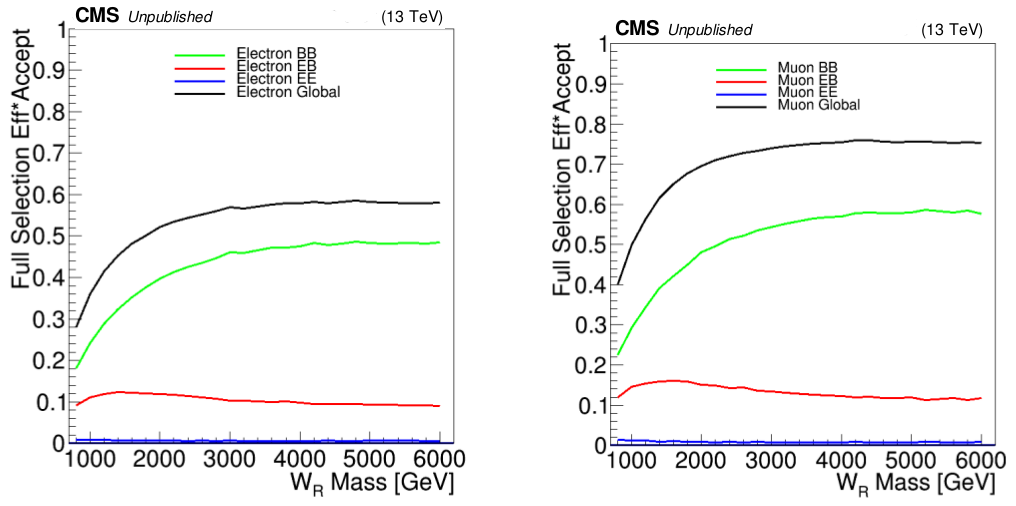
\includegraphics[width=1.0\textwidth]{figures/wrRecoSelectionEfficiency.png}
	\caption{The full selection efficiency in $\WR \rightarrow \ell\ell jj$ events, in the $ee$-channel ($\mu\mu$-channel) 
		on the left (right).  Different curves represent events where both leptons are in the barrel (BB), one was in the 
	endcap (EB), or both were in the endcap (EE).}
	\label{fig:wrRecoSelectionEff}
\end{figure}

After all selections, an excess over expected background events in any kinematic variable distribution 
is evidence of \WR and \nul production.  However, for different variables the excess's shape and magnitude have different 
sensitivities to the unknown ratio $\mnul / \mWR$, and unconstrained parameters of LRS models.  To minimize sensitivity 
to unknown quantities, the $\Mlljj$ variable was chosen as the figure of merit; an example of its discriminating power 
is shown in Figure \ref{fig:mlljjVariableOfMerit}.  The $\Mlljj$ distribution for ST backgrounds was estimated using 
techniques discussed next.

\begin{figure}[h]
	\centering
	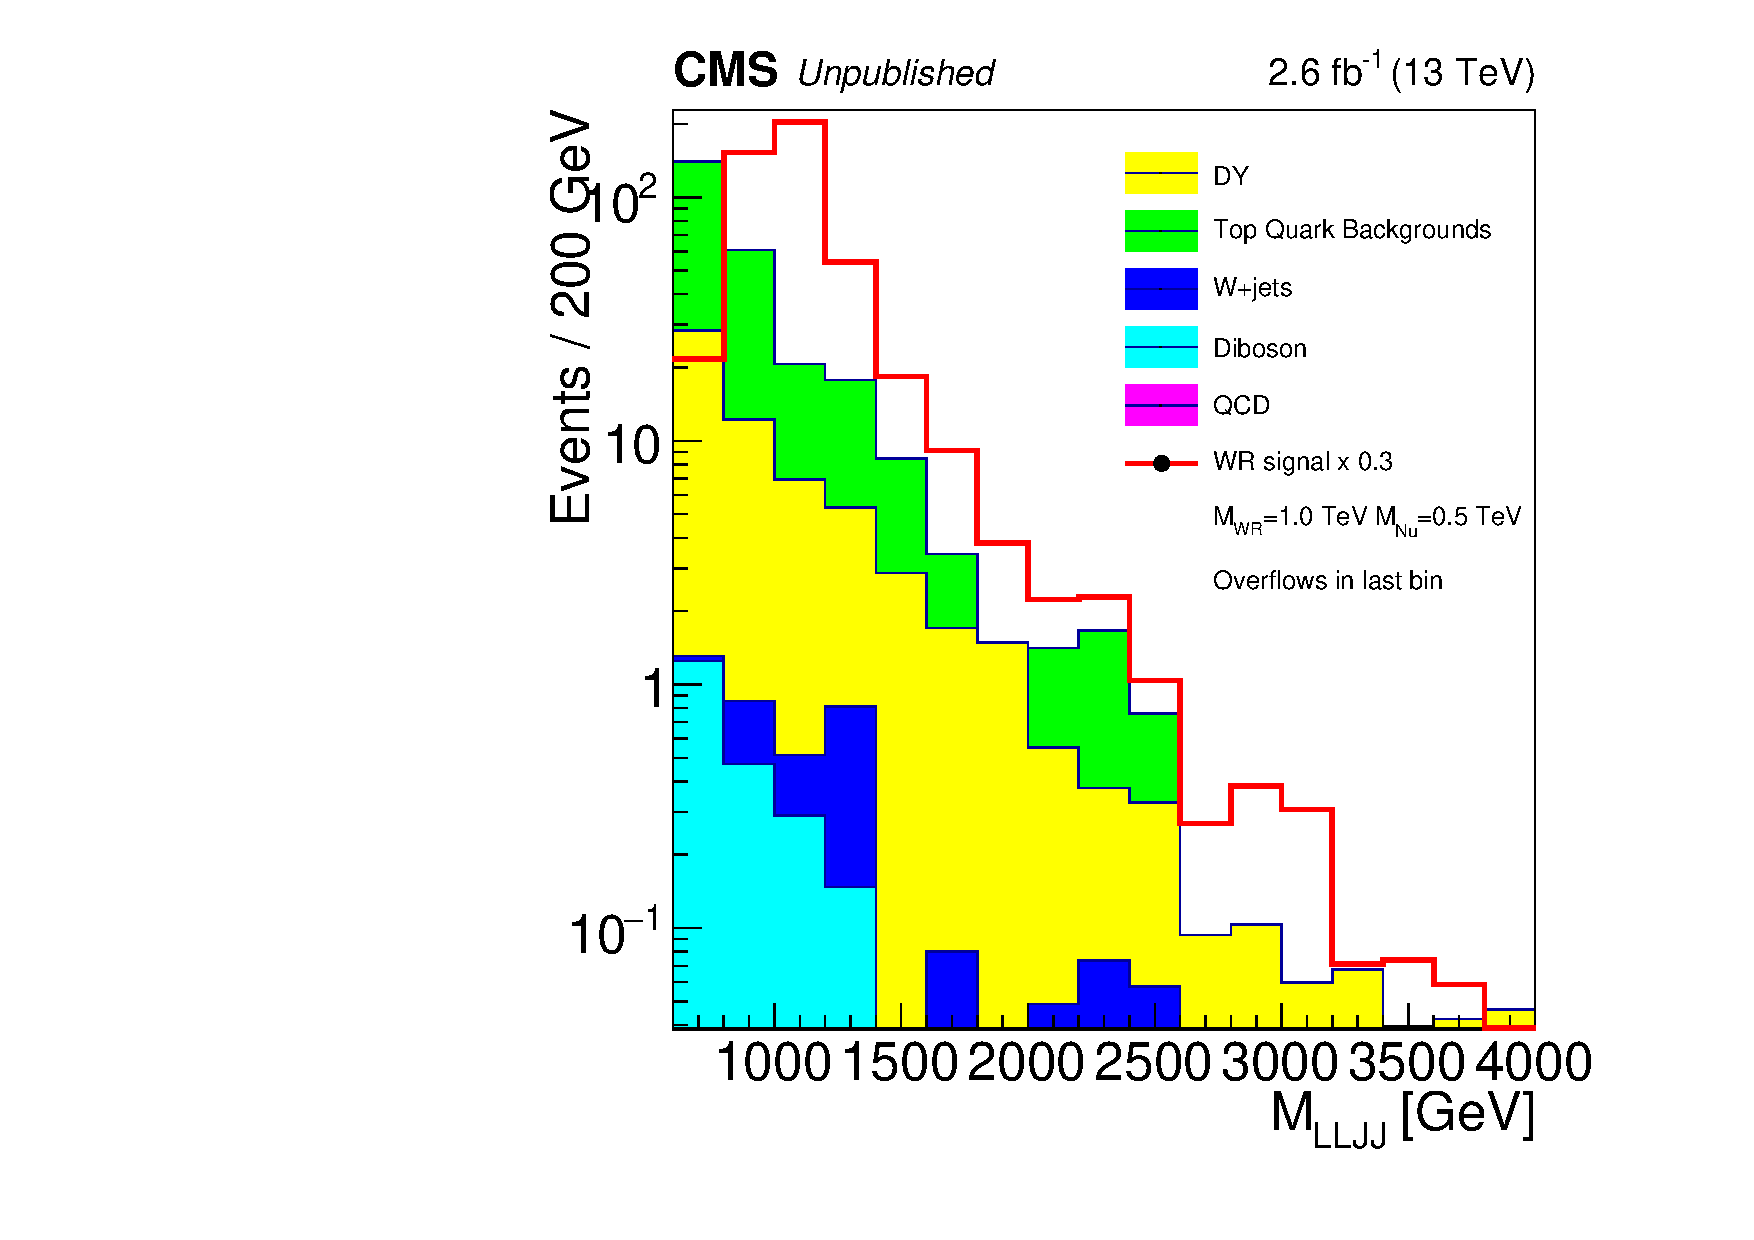
\includegraphics[width=0.7\textwidth]{figures/useOfLLJJMassAsFigureOfMerit.pdf}
	\caption{The $\Mlljj$ distribution from simulations of ST backgrounds and a \WR signal in the $ee$-channel.  
		The \WR signal normalization is reduced by 70\% to better visualize the difference 
	between signal and expected backgrounds.}
	\label{fig:mlljjVariableOfMerit}
\end{figure}


%%%%%%%%%%%%%%%%%%%%%%%%%%%%%%%%%%%%%%%%%%%%%%%%%%%%%%%%%%%%%%%%%%%%%%%%%%%%%%%%
